\documentclass[dvipdfmx]{jsarticle}
% \usepackage{subfigure}
\usepackage{graphicx}
\usepackage{multicol}
\usepackage{float}
\usepackage{circuitikz}
\usepackage{tikz}
\usepackage{amssymb}
\usepackage{arydshln}
\usepackage{wrapfig}
\usepackage{url}
\usepackage{amsmath}
\usepackage{mathtools}
\usepackage{Tabbing}

\newcommand{\undercolor}[2][orange]{
  \textcolor{#1}{\underline{
    \textcolor{black}{#2}
  }}
}

\begin{document}
\title{コンピュータネットワーク}
\date{}
\author{}
\maketitle

\section{コンピュータネットワーク概観}

\subsection{コンピュータネットワークの構成}

\subsubsection{インターネットの構成}

\begin{itemize}
  \item エンドシステム (end system)
  \begin{itemize}
    \item ネットワークに接続しているコンピュータ
    \item ホストともいう
    \item クライアントとサーバに分類されることが多い
  \end{itemize}
  \item クライアント\\
    サービス要求を出す
  \item サーバ\\
    サービス要求を待ち受ける
  \item 通信リンク\\
    光ファイバ、電波、同軸ケーブル、etc...
  \item ルータ\\
    パケットの中継装置
  \item \textcolor{cyan}{ここまでがモノ}
  \item プロトコル\\
    二つ以上の通信エンティティ間でやりとりされるメッセージの形式と順序などを取り決める規約\\
    \textcolor{cyan}{ネットワークの機器間でのやり取りにおけるルール}
\end{itemize}

\newpage
\subsubsection{通信サービス}

エンドシステム間で情報をやり取りするための仕掛け
\begin{itemize}
  \item \textcolor{orange}{コネクション指向型サービス}\\
    クライアントとサーバは、通信を始める前に相互に制御パケットを送信\\
    \textcolor{cyan}{通信前にハンドシェイク}
    \begin{itemize}
      \item \textcolor{orange}{高信頼データ転送}\\
        順序通り、誤りなく伝送
      \item \textcolor{orange}{フロー制御}\\
        受信側のバッファを溢れさせない\\
        \textcolor{cyan}{空きバイト数をフィードバック}
      \item \textcolor{orange}{輻輳制御}\\
        ネットワークの混雑を防ぐ
    \end{itemize}
    代表的なプロトコルは、TCP (Transmission Control Protocol)
  \item \textcolor{orange}{コネクションレス型サービス}\\
    事前の制御パケットのやり取りなしにいきなりデータを送る\\
    代表的なプロトコルは
    \begin{itemize}
      \item UDP (\textcolor{orange}{User Datagram Protocol})
      \item リアルタイムアプリケーション向き
      \item 高い自由度をもつ
    \end{itemize}
    \textcolor{cyan}{高信頼性が無駄なときや、トランスポート層をアプリケーションからいじることができる(TCPをいじりたければOSアップデートが必要)}
\end{itemize}

\newpage
\subsection{ネットワークコア}
エンドシステム間の相互接続を担うルータ群


\subsubsection{回線交換}
エンドシステム間の通信のために経路に沿った通信資源(バッファや帯域の一部)をセッション中常時常時占有

\textcolor{cyan}{予め通信経路を予約して占有}


\subsubsection{パケット交換}
パケット(oacket)
\begin{itemize}
  \item アプリケーションレベルのメッセージを分割したもの
  \item ネットワークコアでの伝送単位
\end{itemize}
\underline{蓄積交換伝送}
\begin{itemize}
  \item 各ルータで到着したパケットを一旦、バッファへ格納
  \item 予め定められた順序(先着順など)に従い、順次パケットを伝送
\end{itemize}

\subsubsection{回線交換 vs パケット交換}

パケット交換の長所
\begin{itemize}
  \item 伝送容量を効率的に利用可能
  \item 実装が容易 \textcolor{cyan}{ルータに送るだけ}
\end{itemize}

回線交換の長所
\begin{itemize}
  \item 通信品質が安定、リアルタイムアプリケーション向き\\
  \textcolor{cyan}{通信を占有するため、安定性が求められるとき}
\end{itemize}

\begin{table}[h]
  \centering
  \caption{回線交換とパケット交換の長所}
  \label{tab:packet}
  \begin{tabular}{c|l|l}\hline
    & 回線交換 & パケット交換\\\hline
    長所
    & \begin{tabular}{c}
        通信品質が安定\\
        リアルタイムアプリケーション向き
      \end{tabular}
    & \begin{tabular}{c}
      伝送容量を効率的に利用可能\\
      実装が容易
    \end{tabular}\\\hline
  \end{tabular}
\end{table}

\newpage
\subsubsection{遅延とパケット損}

各ノード(ルータ)における遅延

\begin{itemize}
  \item 処理遅延: パケットのヘッダを読み、出力リンクを決定する時間\\
    伝送誤りチェックも含む\\
    (通常 $ns \sim \mu s$ のオーダ)\\
    \textcolor{cyan}{パリティチェック等}
  \item 待ち行列遅延: 送信待ちに要する時間\\
    (通常 $100ms$ 程度まで、バッファサイズに依存)\\
    \textcolor{cyan}{LAN出力ポートに複数の出力が来た際の待ち時間、バッファサイズによってパケットを保持できる(より情報を保持できるが待ち時間も増える)}
  \item 伝送遅延: パケットを通信リンクに送り出す時間\\
    (リンクの容量を $R[\rm{bps}]$, パケットサイズを $L\; \rm{bit}$ とすると, $\displaystyle \frac{L}{R}$)
  \item 伝搬遅延: 送信された 1 ビット目の情報が次のノードに到達するまでの時間\\
    (光速より少し遅め、 $2 \times 10^8 m/s \sim 3 \times 10^8 m/s$ 程度)\\
    \textcolor{cyan}{ex.) 衛星通信など。送信元と送信先の距離によって変化}
\end{itemize}
\underline{パケット損}

待ち行列(バッファ)に入ることのできるパケットの数は有限
\begin{itemize}
  \item[$\Rightarrow$] パケット損が生じる
\end{itemize}
一般に、「バッファサイズ大」 $\Leftrightarrow $ 「待ち行列遅延大 かつ パケット損小」\\
というトレードオフが存在

\textcolor{cyan}{パケットの損失はTCPの場合、輻輳制御によってサービスが低下する}


\subsubsection{ルーチング}

送信ホストは終点ホストのアドレス(IPアドレス)をパケットのヘッダに書き込んで送信

ルータは、終点アドレスを出力リンクに対応付けた \textcolor{orange}{ルーチングテーブル} を持ち、検索して転送

\indent\indent\textcolor{cyan}{ネットワークグラフの情報を持っていて、適切な経路を返すイメージ?}

ルータはコネクション情報を管理しない(ヘッダに書かれたアドレスを読むだけ)

ルーチングテーブルの自動作成
\begin{itemize}
  \item[$\Rightarrow$] \textcolor{orange}{ルーチングプロトコル}
\end{itemize}
% フォアディング、アドレッシング

\newpage
\subsubsection{ネットワークのネットワーク}
インターネット (the Internet) は、複数の ISP 同士が階層的に接続することで構成

\indent\textcolor{orange}{ネットワークのネットワーク (Network of network)}

\textcolor{cyan}{イントラネット(企業内などの閉じたインターネット)、ARPANETから始まったインターネットが大きな塊になっていった}

\begin{itemize}
  \item アクセスISP: DSL, FTTH, Wi-Fi, セルラ, ビジネスLANなどによるエンドシステムからのアクセスを提供\\
    \textcolor{cyan}{DSL: 日本では ADSL(asymmetric DSL)}
  \item Tier1 ISP: 他の Tier1 ISPおよび下位ISPと接続し、国際的エリアをカバー\\
    \textcolor{cyan}{日本ではNTTコミュニケーションズとソフトバンクの2社}
  \item Tier2 ISP(広域), Tier3 ISP(地域):
  \begin{itemize}
    \item[] Tier2 ISPは、グローバル通信を行うとき、Tier1 ISPを介してトランジット通信
    \item[] 上位ISPはサービスプロバイダ、下位ISPはカスタマーという関係となり、トラヒック量に応じて料金を課す(従量課金)
  \end{itemize}
  \textcolor{cyan}{ISP: Internet survice provider, 通信の企業のことみたい。kddi $\rightarrow$ so-net $\rightarrow$ user みたいな感じ?}
\end{itemize}

\begin{itemize}
  \item ピアリング:
  \begin{itemize}
    \item[] 同層ISP間で接続すること。
    \item[] 上位ISPへのトランジット料金の支払いを軽減
  \end{itemize}
  \item  相互接続点(PoP: Point of Presence): ISP間が接続するときの接続点\;(複数のルータから構成)\\
  \textcolor{cyan}{複数の事業者間で通信するには物理的にルータが繋がっている必要がある}
  \item IXP(Internet Exchange Point): ピアリングするISPがつなぎこむ箇所を提供する、独立した組織\\
  \textcolor{cyan}{PoPを提供する事業者}
  \item コンテンツプロバイダ:
  \begin{itemize}
    \item Googleなど、非常に大きなリソースを持つサードパーティ (\textcolor{orange}{Hypergiants}などとも呼ばれる)
    \item Tier2, Tier3 ISP と直接ピアリングを行う
    \item[] \textcolor{cyan}{従量課金がなくなるため、下位ISPとしてもWin-Win}
  \end{itemize}
\end{itemize}

\begin{figure}[h]
  \centering
  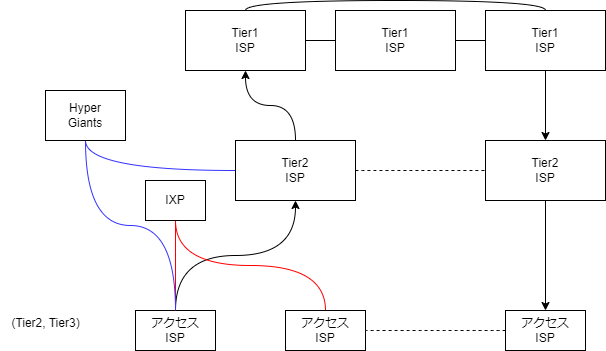
\includegraphics[width=0.6\linewidth]{image/isp.png}
  % \caption{}
  % \label{fig:}
\end{figure}

\newpage
\subsection{プロトコル階層とサービスモデル}

\subsubsection{階層化アーキテクチャ}

インターネットは極めて複雑なシステム
\begin{itemize}
  \item[] プロトコルならびに、それを動作させるハードウェア、ソフトウェアを階層化して設計
  \begin{itemize}
    \item[$\Rightarrow$] ネットワーク設計の複雑さを軽減し、各構成要素間の役割や関係を明確にする
    \item[] \textcolor{cyan}{モジュール化、個別に設計}
  \end{itemize}
\end{itemize}

各プロトコルはある一つの階層(layer)に属する
\begin{itemize}
  \item[] 第n層のプロトコルは第n層同士でメッセージを交換
  \begin{itemize}
    \item[] 第n層のプロトコルデータユニット(n-PDU): 第n層で交換されるメッセージ
  \end{itemize}
\end{itemize}

\begin{itemize}
  \item プロトコルスタック(protocol stack): これらのプロトコルが構成する階層全体
  \begin{itemize}
    \item[$\cdot$] OSI参照モデル(Open System Interconnection Refference Model): 7層構造
    \item[$\cdot$] インターネット(TCP/IP): 5層構造
  \end{itemize}
\end{itemize}

\begin{figure}[h]
  \centering
  
\includegraphics[width=0.8\linewidth]{image/npu.png}
\end{figure}


ホストAの第n層がホストBの第 n 層にn-PDUを送信
\begin{enumerate}
  \item ホストAの第n層がホストBの第 $n-1$ 層にn-PDUを渡し、ホストBの第n層への送信を依頼
  \item 第n層は第 $n-1$ 層のサービスを受ける  (第 $n-1$ 層は第n層にサービスを提供)
  \item 第n層は第 $n-1$ 層がどのようにサービスを実現しているかを意識しない
  \begin{itemize}
    \item[$\Rightarrow$] 層間のインターフェースが定義されていれば差し替え可能
    \item[] \textcolor{cyan}{抽象メソッドみたい}
  \end{itemize}
  \item[] \textcolor{cyan}{層が深くなるにつれ、誤り訂正などの処理が行われる}
\end{enumerate}


$\cdot$ プロトコル階層化の欠点
\begin{itemize}
  \item 同じ機能を複数の層が持つ場合がある (誤り制御など)
  \begin{itemize}
    \item[] \textcolor{cyan}{データ量的に無駄}
  \end{itemize}
  \item 上位層は下位層の情報を利用できない (柔軟性の欠如)
\end{itemize}


\newpage
\subsubsection{インターネットプロトコル階層}

\begin{table}[h]
  \centering
  \caption{}
  \label{tab:}
  \begin{tabular}{c|c|c}
    && PDUの呼び方\\\hline
    Layer 5 & アプリケーション & メッセージ \\
    Layer 4 & トランスポート & セグメント\\
    Layer 3 & ネットワーク データグラム(パケット)\\
    Layer 2 & データリンク & フレーム\\
    Layer 1 & 物理 & 1-PDU\\\hline
  \end{tabular}
\end{table}

\begin{itemize}
  \item アプリケーション層\\
    \underline{ネットワークアプリケーションをサポート}
  \begin{itemize}
    \item[例)] HTTP: web
    \item[] SMTP: 電子メール
    \item[] FTP: ファイル転送
  \end{itemize}
  \item トランスポート層\\
    \underline{アプリケーションプロセス間}のメッセージ転送サービスで提供
  \begin{itemize}
    \item TCP: 高信頼データ転送、フロー制御、輻輳制御
    \item UDP: コネクションレス型サービス
  \end{itemize}
  \item ネットワーク層\\
    始点・終点ホスト間でデータグラムの転送を行うIP・インターネットの3層プロトコル (IP層ともいう)
  \begin{itemize}
    \item[] IPデータグラムの定義と、それに基づくエンドシステムやルータの動作を規定
    \item ルーチングプロトコル:\\
      始点ホストから終点ホストまでの経路を設定\\
      複数のプロトコルが存在
    \end{itemize}
  \item データリンク層\\
    \underline{ノード間の1ホップ} の通信を担う
  \begin{itemize}
    \item[例)] Wi-Fi, イーサネット(有限LAN)など
  \end{itemize}
  \item 物理層
  \begin{itemize}
    \item フレーム内の各ビットを伝送
    \item \begin{tabbing}
      物理メディア: \=より対線、同軸ケーブル\\
      \>光ファイバ、無線など
    \end{tabbing}
  \end{itemize}
\end{itemize}

ネットワークエンティティ

\indent\indent ネットワークの構成要素(エンドシステムと中継器)
\begin{itemize}
  \item \begin{tabbing}
    中継器: \=ルータ(3層まで)\\
    \>ブリッジ、スイッチ(2層まで)
  \end{tabbing}
  \item エンドシステム: 5層すべて
\end{itemize}

\newpage
\section{アプリケーション層プロトコル}

\subsection{基礎}
\subsubsection{アプリケーション層プロトコル}

\begin{itemize}
  \item ネットワークアプリケーション: ネットワークの使用を前提とするソフトウェア
  \begin{itemize}
    \item[例)] Webアプリケーションは、ブラウザ(Chrome, Safariなど) とWebサーバ (Apacheなど) の複数のソフトウェアから構成
    \item[] \textcolor{cyan}{Webサーバは他にも nginxとか}
  \end{itemize}
\end{itemize}

\begin{itemize}
  \item アプリケーション層プロトコルは。メッセージ交換方法やメッセージのタイプ・フォーマットを規定
  \begin{itemize}
    \item[例)] webでは HTTP を使用
  \end{itemize}
  \item ネットワークアプリケーションは一般にクライアントとサーバの両方の側面をもつ (WebブラウザとWebサーバの関係)
  \item ネットワークを介した \textcolor{orange}{プロセス間通信}
  \item[] \textcolor{cyan}{プロセス間通信は実際には1つ下の層であるトランスポート層が提供 (自由度が高いらしい)}
  \begin{itemize}
    \item 二つのエンドシステムにあるプロセス間でネットワークを介してやり取り
    \item ソケット (Socket) と呼ばれる仮想的なインターフェースを用いる
    \begin{itemize}
      \item ソケットはAPI (Application Programming Interface) の一種
      \item トランスポート層とのインターフェースの役割
    \end{itemize}
  \end{itemize}
  % 黒板の改ページ
  \item コネクション (フロー) の単位
  \begin{itemize}
    \item[※] アプリケーション層が割り当てる情報
    \begin{itemize}
      \item 送受信ホストの \undercolor{IPアドレス}  % 1, 2
      \item プロセスの送受信 \undercolor{ポート番号} % 3, 4
      \begin{itemize}
        \item[$\rightarrow$] ホストのどのプロセスかを特定する番号
      \end{itemize}
      \item サーバ側プロセスは多くの場合ポート番号が固定
      \begin{itemize}
        \item 1023番まではwell-knownポートとして予約 (HTTP:80. SMTP:25, DNS:53 など)
      \end{itemize}
    \end{itemize}
  \end{itemize}
  \item トランスポート層プロトコル \undercolor{(TCP, UDP)}  % 5
  \item[] \textcolor{cyan}{同じポート番号でもプロトコルが違えば使用可能}
\end{itemize}
% 1,2,3,4,5 をまとめてなんか言ってた
% 5個情報送るよって話

\newpage
\subsubsection{トランスポート層プロトコルから提供されるサービス}

アプリケーション製作者は、「データ損失」「帯域幅」「遅延」の観点から選択

\begin{itemize}
  \item TCPサービス
  \begin{itemize}
    \item コネクション指向型: 全2重コネクション。ハンドシェイクを待ってから通信
    \item 高信頼データ伝送: 誤りのない、正しい順序のデータ送信を保証
    \item 輻輳制御: ネットワークの混雑に合わせて伝送レートを変更
  \end{itemize}
  \item UDPサービス
  \begin{itemize}
    \item 最小限のデータ伝送: メッセージの到達性や正確性は保証しない
    \item コネクションレス型: ハンドシェイクは行わない
    \item 輻輳制御なし: 伝送レートは始点プロセスで指定
  \end{itemize}
\end{itemize}

\subsubsection{アプリケーション層プロトコルの分類}

プル型、プッシュ型
\begin{itemize}
  \item プル型プロトコル
  \begin{itemize}
    \item HTTP, FTPなど
    \item ユーザが必要に応じて情報を引き出す (サーバが情報通信)
    \item 情報取得を希望するクライアントがコネクションを開始
    \end{itemize}
  \item プッシュ型プロトコル
  \begin{itemize}
    \item SMTPなど: (メールを送る側が相手へ情報送信)
    \item 情報発信する側がコネクションを開始
  \end{itemize}
\end{itemize}

個別帯域、共通帯域
\begin{itemize}
  \item 個別帯域 (out-of-band) 方式
  \begin{itemize}
    \item 制御用とデータ用で別のコネクションを使用\\
    \textcolor{cyan}{大きなファイルのアップロードの際に制御情報を別ルートで送ることができる}
    \item 代表例はFTP \textcolor{cyan}{Webページの更新など}
  \end{itemize}
  \item 共通帯域 (in-band 方式)
  \begin{itemize}
    \item 制御用とデータ用で同じコネクションを使用
      \textcolor{cyan}{(TCPを想定)}
    \item 代表例はHTTP
  \end{itemize}
\end{itemize}

個別帯域の例
\begin{itemize}
  \item 個別帯域の考え方は色々な場合に存在
  \item OpenFlow
  \item 5GのC/U 分離 (フェムトセル) \textcolor{cyan}{control, user \url{https://jirei.bzlog.jp/5g/information_14/}}
  \begin{itemize}
    \item マクロセルで制御信号をやり取り
    \item フェムトセルで高速データ転送
  \end{itemize}
\end{itemize}

\newpage
\subsection{WebとHTTP}
\subsubsection{HTTPの概要}

\begin{itemize}
  \item HTTP(Hypertext Transfer Protocol):\\
    Web用のアプリケーション層プロトコル
  \item Web ページ:\\
    基本となるHTMLファイルと、いくつかのWebオブジェクトの集合体\\
    URLにはホスト名やパス名、ファイル名が含まれる
  \item Webオブジェクト: HTMLファイル, 各種画像, JavaScript, 音声データ, 動画など
  \item Webブラウザ: Webページを表示するHTTPクライアント(Chrome, Safari, Edge, Firefox など)
  \item Webサーバ: Webオブジェクトを蓄えるHTTPサーバ(Apacheなど)
\end{itemize}

\begin{itemize}
  \item HTTPは、WebブラウザがWebサーバに対しWebページを要求する方法やサーバがそれに対して返送するための方法を定義
  \begin{itemize}
    \item 基本的に、クライアントがHTTP requestメッセージを送り、サーバがHTTP responseメッセージを返す % 板書だとresponce: たいぽ?
  \end{itemize}
  \item トランスポート層プロトコルはTCP\\
    (ソケットに渡したあとは到達性が保証される)
  \begin{enumerate}  % [(i), (ii), (iii), (iv)]
    \item クライアントがサーバのポート 80 へTCPコネクションを要求
    \item サーバとクライアントの間でTCPコネクションを確立
    \item HTTPメッセージをクライアント・サーバ間で交換
    \item TCPコネクションをクローズ
  \end{enumerate}
\end{itemize}

\begin{itemize}
  \item HTTPはステートレス(stateless)なプロトコル
  \begin{itemize}
    \item サーバはクライアントの履歴情報を記憶しない\\
      例えば同じクライアントから、同じ要求が2回届くとサーバは同じレスポンスを2回返す
    \item 制御が軽く、同時に多数のHTTP要求に対応可能\\
      状態を記憶する場合、状態の維持や故障・切断時の処理定義が別途必要
  \end{itemize}
  \textcolor{cyan}{ステートレス:履歴をもたない (一昔前のチャットボットみたいな感じ?)}\\
  \textcolor{cyan}{webの情報はクライアント側が保持(cookie?)}
\end{itemize}

\subsubsection{非継続型コネクションと継続型コネクション}

\begin{itemize}
  \item 非継続型コネクション( non-persistent connection)
  \begin{itemize}
    \item 一つのTCPコネクションは一つのWebオブジェクトを転送
    \item 通常ブラウザは並列して5から10のTCPコネクションをはれるが埋まっていれば、各オブジェクトは直列に処理される
    \item HTTP/1.0で使用
  \end{itemize}

  \begin{itemize}
    \item 非継続型の欠点
    \begin{itemize}
      \item 多くのTCPコネクションをサーバが管理する必要
      \item 各オブジェクトの転送に、2RTT必要(TCPコネクションの確立に1RTT要する)
      \item[] ※ RTT(Round Trip Time: 往復遅延時間)
    \end{itemize}
  \end{itemize}
\end{itemize}

\begin{itemize}
  \item 継続型コネクション(Persistent connection)
  \begin{itemize}
    \item 一つのコネクションで複数のWebオブジェクトを転送
    \item サーバは応答を返した後もTCPコネクションを継続
    サーバで認定された一定時間(タイムアウト時間)使用されたなければコネクションを切断
    HTTP/1.1 のデフォルト
  \end{itemize}
\end{itemize}

パイプライン処理
\begin{itemize}
  \item 非パイプライン処理型 (without pipelinig)
  \begin{itemize}
    \item クライアントは応答メッセージの受信を待ってから、次の要求メッセージを送信
  \end{itemize}
  \item パイプライン処理型 (with pipelinig)
  \begin{itemize}
    \item クライアントは応答メッセージを受け取るまえに、次々と要求メッセージを送信可能
  \end{itemize}
\end{itemize}

\subsubsection{HTTPメッセージ}

\begin{itemize}
  \item 2種類のメッセージ: リクエスト(要求), レスポンス(応答)
  \item HTTPリクエストメッセージ
  \begin{itemize}
    \item \begin{tabbing}
      リクエスト行: \=HTTPメソッド(GET, POSTなど)\\
      \>リクエスト対象(URL) \\
      \>HTTPバージョン
    \end{tabbing}
    \item ヘッダ行   : user agent などを key:value形式でストア
    \item 本文
  \end{itemize}
  \item HTTP応答メッセージ
  \begin{itemize}
    \item \begin{tabbing}
      ステータス行: \=ステータスコード(200, 403, 404, 503など)\\
      \> ステータス文字列(OK, Permission Denied, Not Found, Service Unavailable など)
    \end{tabbing}
    \item ヘッダ行: ViaやContent-lengthなどを key:value形式でストア
    \item 本文
  \end{itemize}
\end{itemize}


\end{document}
